\documentclass{article}
\usepackage[utf8]{inputenc}
\usepackage{hyperref}
\usepackage{graphicx}
\usepackage{amssymb}
\title{CSC412 Notes Week 3}
\author{Jerry Zheng}
\date{April 2021}
\hypersetup{
    colorlinks=true,
    linkcolor=blue,
    filecolor=magenta,      
    urlcolor=blue,
    pdftitle={Sharelatex Example},
    bookmarks=true,
    pdfpagemode=FullScreen,
}

\begin{document}

\maketitle

\section{Graphical Models}
\subsection{Chain Rule}
The joint distribution of (N) random variables can be evaluated with the chain rule\\

$$P(x_{1, ..., N}) = P(x_1)P(x_2|x_1)P(x_3 | x_2, x_1) \ldots P(x_n | x_{n-1 ,..., 1})$$\\

When we have a joint distribution of discrete random variables with full dependence between variables.\\

More formally, in probability the chain rule for two random variables is\\
$$P(x, y) = P(x | y)P(y)$$\\

\subsection{Conditional Independence}

To represent large joint distributions we can assume conditional independence
$$X \perp Y | Z \Leftrightarrow P(X, Y | Z) = P(X | Z)P(Y | Z) \Leftrightarrow P(X | Y, Z) = P(X | Z)$$
This is very useful as now we can represent a large chain of N variables as a product of independent variables.
$$P(x_{1:n})  = P(x_1) \prod_{t=1}^n P(x_t|x_{t-1})$$

this is the (first order) Markov Assumption. Where "the future is independent of the past given the present"

\subsection{Probabilistic Graphical Models}
If you don't know what a  graph is, \href{https://en.wikipedia.org/wiki/Graph_(discrete_mathematics)}{Wikipedia}\\

A probabilistic graphical model can modeled can be used to represent joint distributions when we assume Conditional Independence. In this model, nodes are variables and edges show conditional dependence.\\

\subsection{Directed Acyclical Graphical Model}
Using the Markov Assumption  we can very easily represent complicated graphs.\\
A 4 node starting graph can be represented with half the number of edges!\\
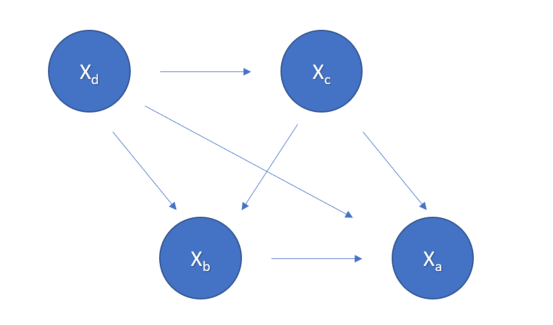
\includegraphics[scale=0.7]{Screenshot_2.png}\\

can now be represented as\\
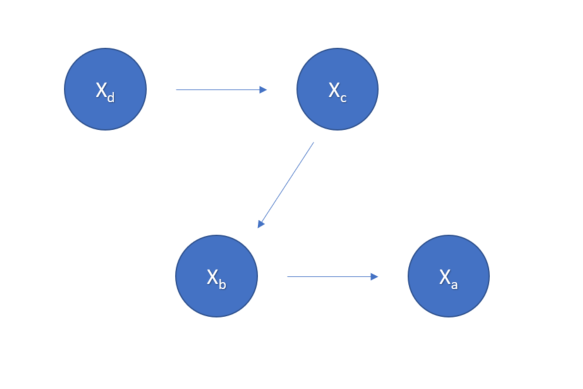
\includegraphics[scale=0.7]{Screenshot_3.png}\\

its easy to see that $X_a$ is much easier to evaluate in the second graph than the first.

$$P(x_a) = P(x_a| x_b, x_c, x_d) P(x_b| x_c, x_d )P( x_c | x_d) P(x_d)$$
can be simplified to this with the Markov assumption.
$$P(x_a) = P(x_a| x_b) P(x_b| x_c)P( x_c | x_d) P(x_d)$$

\section{Conditional Independence and Directed-Separation }
Directed-separation is where two variables in a DAGM may or may not be connected given a third variable.\\
D-connection implies conditional dependence.\\
D-separation implies conditional independence.\\
\\
This also extrapolates into groups/sets of variables for X Y Z

$$X = \{X_1, ...X_n\}$$
$$Y = \{Y_1, ...Y_n\}$$
$$Z = \{Z_1, ...Z_n\}$$
$$X \bot Z | Y$$\\
If every variable in X is d-separated from every variable in Z conditioned on all the variables in Y.\\
To determine d-separation we will use the Bayes ball algorithm\\

For Bayes Ball there are 3 structures that you must know.

\subsection{Bayes Ball - Chain}
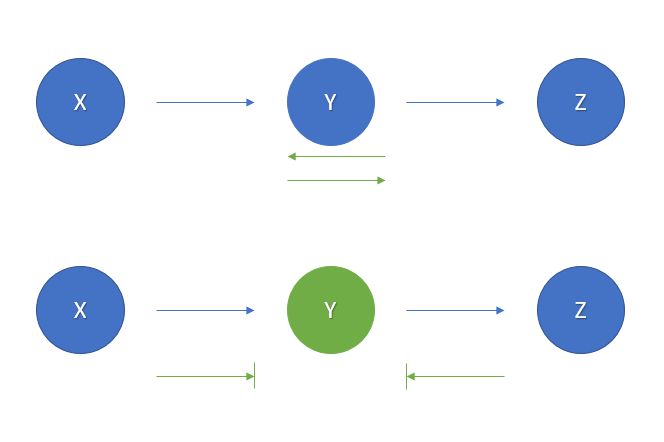
\includegraphics[scale=0.7]{Screenshot_7.png}\\

X and Z are conditionally dependent when y is unknown and conditionally independent when y is known.\\
From the chain's graph, we  can encode the structure as.
$$P(x, y, z) = P(x)P(y|x)P(z|y)$$
once we condition on y we get.
$$
P(x, z | y) = \frac{P(x)p(y|x)p(z|y))}{P(y)} \\
= \frac{P(x, y)P(z|y)}{P(y)} \\
= P(x | y) P(z | y) \\ 
$$
$$\therefore  x \bot z | y$$

\subsection{Bayes Ball - Fork}
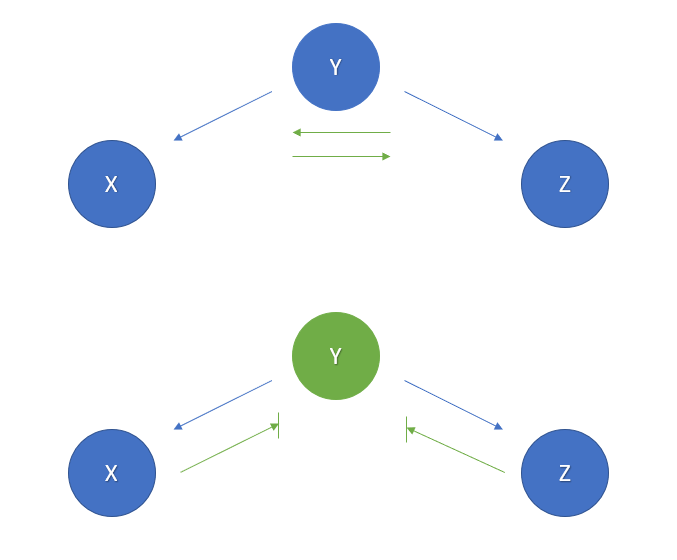
\includegraphics[scale=0.7]{Screenshot_8.png}\\
X and Z are conditionally dependent when y is unknown and conditionally independent when y is known.\\
from the fork's graph we get the equation\\
$$P(x, y, z) = P(y)P(x|y)P(z|y)$$
conditioning on y we get.
$$
P(x, z | y) = \frac{P(x, y, z)}{P(y)} \\
= \frac{P(y)P(x|y)P(z|y))}{P(y)} \\
= P(x | y) P(z | y) \\ 
$$
$$\therefore  x \bot z | y$$

\subsection{Bayes Ball - Collider}
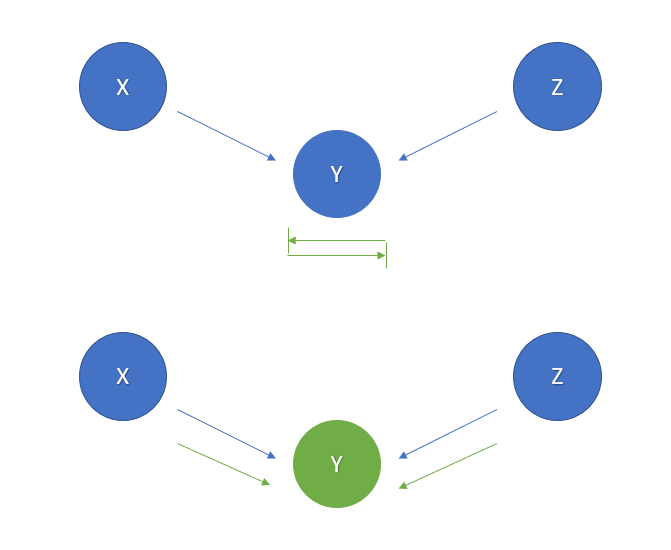
\includegraphics[scale=0.7]{Screenshot_9.png}\\
X and Z are conditionally independent when y is unknown and conditionally dependent when y is known.\\
From the collider's graph we get the equation\\
$$p(x, y, z) = p(x)p(z)p(y|x, z)$$
conditioning on y we get.
$$
P(x, z | y) = \frac{P(x, y, z)}{P(y)} \\
= \frac{p(x)p(z)p(y|x, z))}{P(y)} \\
= P(x) P(z) \\ 
$$
$$\therefore  x \not \perp z | y$$

however if we do not condition on y it's  easy to see that...
$$ P(x, z) = P(x) P(z)$$
$$\therefore  x \perp z$$
So we see that conditioning on a common child at the bottom of a collider/v-structure makes its parents become dependent.\\
This important effect is called explaining away, inter-causal reasoning, or Berkson’s paradox.\\
\\
As an example,\\
$X$ is the event of a Toronto Raptors parade $P(X)=0.01$\\
$Z$ is the event of a car accident $P(Z)=0.1$\\
$Y$ is the event of a traffic jam downtown\\
Lets say that these are the only 2 sources of traffic. So if we know a traffic jam has occurred, then at least one of the two events has happened.\\
\subsection{Boundary Conditions}
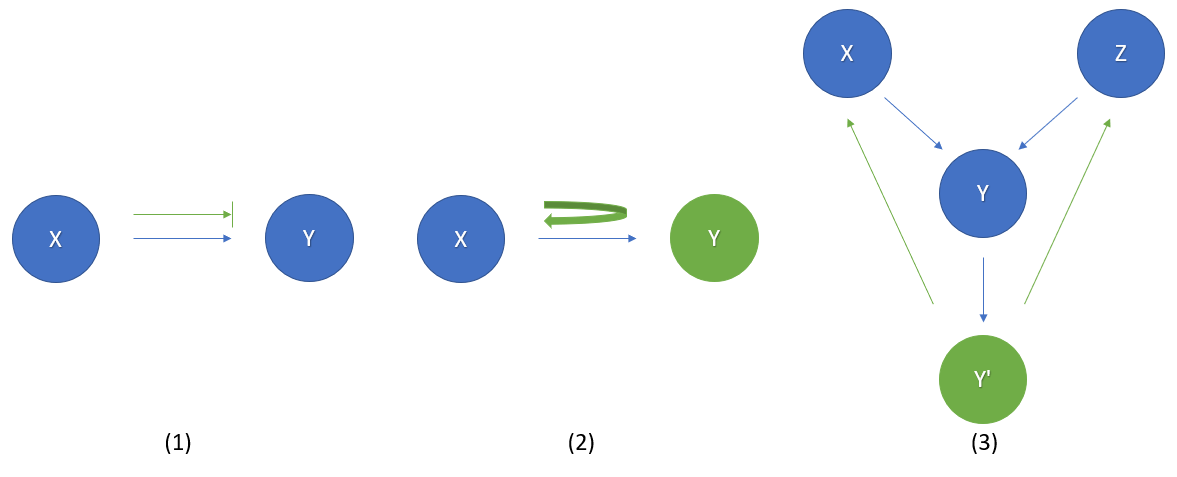
\includegraphics[scale=0.4]{Screenshot_11.png}\\
In example 3, if any child of Y is observed then Y is effectively observed, so the information 'bounces back'.\\
This is shown again in examples 1 and 2. Where if Y is known then the information goes up the chain.\\
\pagebreak
\subsection{Putting It Together}
Now that we understand Conditional Independence with Bayes Ball on simple graphs we can apply this to complex graphs.\\
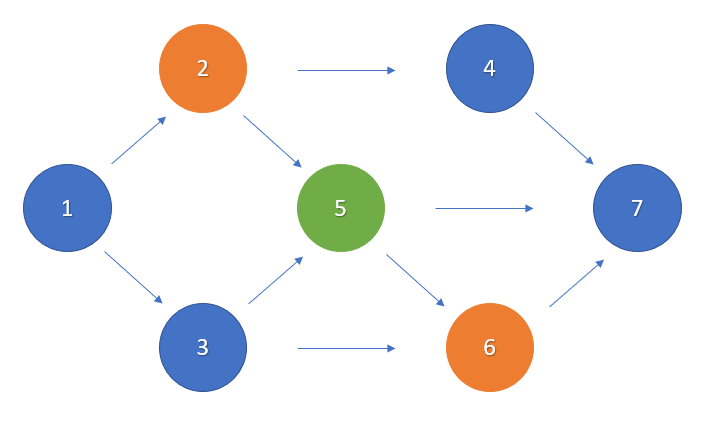
\includegraphics[scale=0.7]{Screenshot_10.png}\\
Say, we want to determine the conditional dependence of 2 and 6 given 5.\\
There are 3 paths from 2 to 6. \\
2 → 5 → 6 cannot be traversed $2\perp 6 | 5$ (known chain)\\
2 → 4 → 7 → 6 cannot be traversed $4 \perp 6 | 7$ (unknown collider)\\
2 → 1 → 3 → 6 cannot be traversed $2 \perp 3 | 1$ (unknown fork)\\
so we can say $2 \perp 6 | 5$.\\
This would change if we knew 1 or 6 or didn't know 5.
\end{document}
